\chapter{Estrategia de síntesis y química verde}\label{ch:g12:synthesis-strategy}

El mismo analgésico, el ibuprofeno, se ha fabricado de dos maneras. La
ruta más antigua tiene seis etapas, y de cada cien kilos de \omterm{def:g5:raw-materials-and-recycling:raw-material}{materias
primas} que compra, sesenta acaban como residuos. La más reciente tiene
tres etapas y conserva casi todos los \omterm{def:g7:atoms-and-molecules:atom}{átomos} que compra. Las dos dan el
mismo polvo blanco del comprimido; se diferencian en la planificación.
Un químico que planifica una \omterm{def:g10:synthesis-yield:synthesis}{síntesis} se hace cuatro preguntas: cómo ir
deprisa, cómo obtener mucho, cómo tocar solo la parte adecuada de una
\omterm{def:g7:atoms-and-molecules:molecule}{molécula} y cómo desperdiciar poco.

\begin{recall}
Una \omterm{def:g10:synthesis-yield:synthesis}{síntesis}: reacción, separación, purificación, identificación; su
\omterm{def:g10:synthesis-yield:yield}{rendimiento} (\cref{ch:g10:synthesis-yield}). Las \omterm{def:g12:curly-arrows:curly-arrow}{flechas curvas}, la
sustitución, la adición, la \omterm{def:g12:curly-arrows:categories}{eliminación} (\cref{ch:g12:curly-arrows}). Un
\omterm{def:g12:catalysis:catalyst}{catalizador} acelera una reacción sin consumirse (\cref{ch:g12:catalysis}).
Una \omterm{def:g12:equilibrium:non-total}{reacción no total} se detiene cuando $Q = K$; un exceso de un
\omterm{def:g7:chemical-reactions:reactant}{reactivo}, o la retirada de un producto, la lleva más lejos
(\cref{ch:g12:equilibrium}).
\end{recall}

\begin{omfigure}
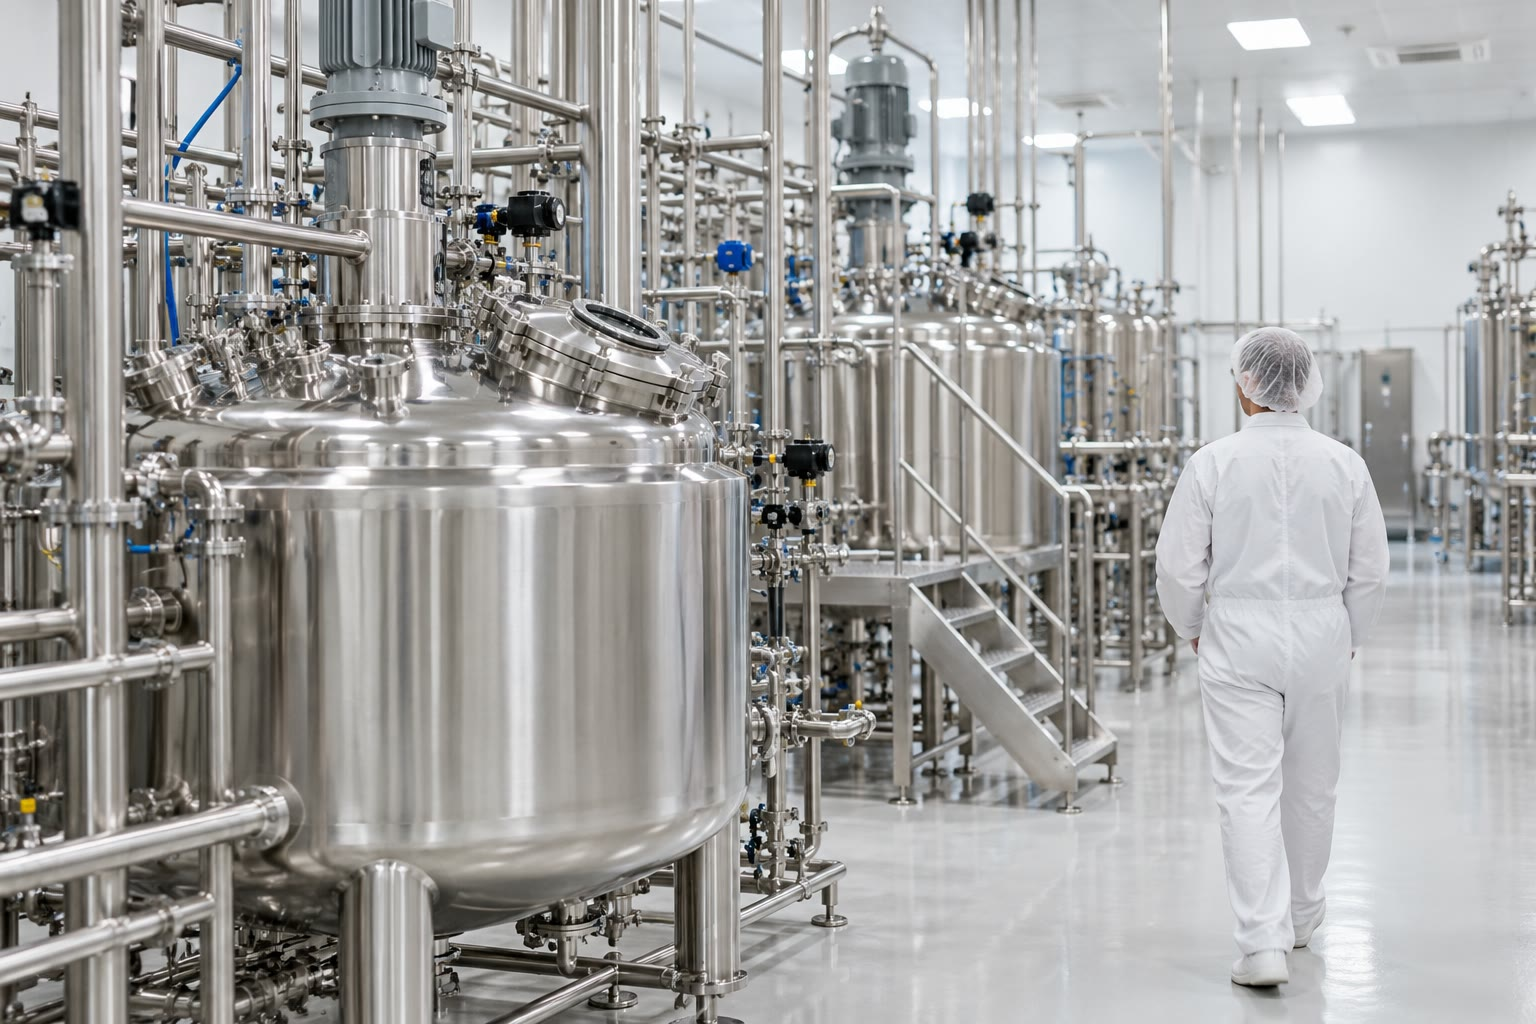
\includegraphics[width=0.48\linewidth]{images/book1/ai/g12-pharma-plant.jpg}

{\small Una planta farmacéutica: los reactores de una \omterm{def:g10:synthesis-yield:synthesis}{síntesis}, a escala
de toneladas.}
\end{omfigure}

\section{Optimizar una síntesis}

Se pueden mejorar dos cosas distintas: la \emph{velocidad}, que decide
cuánto dura la \omterm{def:g10:synthesis-yield:synthesis}{síntesis}, y el \emph{\omterm{def:g10:synthesis-yield:yield}{rendimiento}}, que decide cuánto
producto da.

\begin{proposition}[Palancas sobre la velocidad y el rendimiento]\label{prop:g12:synthesis-strategy:levers}
\begin{itemize}
  \item La velocidad aumenta con la temperatura, con las concentraciones
        de los \omterm{def:g7:chemical-reactions:reactant}{reactivos} y con un \omterm{def:g12:catalysis:catalyst}{catalizador}.
  \item El \omterm{def:g10:synthesis-yield:yield}{rendimiento} final de una \omterm{def:g10:reaction-progress-table:limiting}{reacción total} lo fija el \omterm{def:g10:reaction-progress-table:limiting}{reactivo
        limitante}; el de una \omterm{def:g12:equilibrium:non-total}{reacción no total} aumenta con un exceso de
        uno de los \omterm{def:g7:chemical-reactions:reactant}{reactivos}, o con la retirada de un producto a medida
        que se forma. Un \omterm{def:g12:catalysis:catalyst}{catalizador} no lo cambia: solo lleva el sistema
        más deprisa al mismo \omterm{def:g10:reaction-progress-table:system}{estado final}.
\end{itemize}
\end{proposition}

\begin{proof}
El primer punto reúne los \omterm{def:g12:reaction-rates:kinetic-factor}{factores cinéticos} de los
\cref{ch:g12:reaction-rates,ch:g12:catalysis}. El segundo se deduce de
que $Q = K$ al final de una \omterm{def:g12:equilibrium:non-total}{reacción no total}: añadir un \omterm{def:g7:chemical-reactions:reactant}{reactivo} o
retirar un producto hace que $Q < K$, y la reacción sigue en sentido
directo.
\end{proof}

\begin{example}[Esterificación con trampa de agua]\label{ex:g12:synthesis-strategy:trap}
El ácido etanoico y el etanol, un \omterm{def:g10:the-mole:amount}{mol} de cada uno, solo dan un
\qty{67}{\percent} de \omterm{def:g11:functional-groups:carboxylic-acid}{éster} en el equilibrio. Si la \omterm{def:g6:pure-substances-and-mixtures:mixture}{mezcla} se calienta a
reflujo en un \omterm{def:g6:solutions-and-solubility:solute}{disolvente} que no se \omterm{def:g6:pure-substances-and-mixtures:mixture}{mezcla} con el agua, con un poco de
ácido como \omterm{def:g12:catalysis:catalyst}{catalizador}, el vapor se condensa en un tubo lateral, una
\emph{trampa de agua}: el agua, más densa, se deposita en el fondo y se
queda allí, mientras que el \omterm{def:g6:solutions-and-solubility:solute}{disolvente} vuelve al matraz. El agua sale de
la reacción a medida que se forma, $Q$ se mantiene por debajo de $K$, y
la esterificación llega casi hasta el final. El calentamiento aporta la
velocidad; el \omterm{def:g12:catalysis:catalyst}{catalizador}, más velocidad; y la trampa, el \omterm{def:g10:synthesis-yield:yield}{rendimiento}.
\end{example}

\begin{omfigure}
\begin{tikzpicture}[font=\small, scale=0.8]
  \pic[transform shape] at (0,0) {hotplate};
  \pic[transform shape] at (0,0) {rbflask={0.55}{orange!20}};
  % the trap: water at the bottom, solvent above, up to the arm
  \fill[cyan!60!blue!40] (1.0,1.75) arc[start angle=180, end angle=360, radius=0.15] -- (1.3,2.3) -- (1.0,2.3) -- cycle;
  \fill[yellow!35] (1.0,2.3) rectangle (1.3,3.25);
  \draw[om glass] (-0.2,3.0) -- (-0.2,3.75) -- (0.2,3.75) -- (0.2,3.55) -- (1.0,3.55) -- (1.0,4.0);
  \draw[om glass] (0.2,3.0) -- (0.2,3.25) -- (1.0,3.25) -- (1.0,1.75) arc[start angle=180, end angle=360, radius=0.15] -- (1.3,4.0);
  \pic[transform shape] at (1.15,4.0) {condenser};
  \draw[omProp, thick, <-] (1.35,2.0) -- (2.6,1.7) node[right, text=black, align=left] {el agua se acumula\\ en el fondo};
  \draw[omProp, thick, <-] (1.35,2.9) -- (2.6,3.1) node[right, text=black, align=left] {el disolvente rebosa\\ y vuelve al matraz};
  \draw[omProp, thick, <-] (-0.6,0.6) -- (-1.7,1.1) node[left, text=black, align=right] {ácido, alcohol,\\ catalizador, disolvente};
\end{tikzpicture}

{\small Una trampa de agua sobre un matraz calentado a reflujo: el agua
formada se retira de la reacción a medida que se condensa.}
\end{omfigure}

\section{Selectividad}

Una \omterm{def:g7:atoms-and-molecules:molecule}{molécula} real suele llevar varios \omterm{def:g11:functional-groups:functional-group}{grupos funcionales}. Un \omterm{def:g7:chemical-reactions:reactant}{reactivo} que
los ataca todos da una \omterm{def:g6:pure-substances-and-mixtures:mixture}{mezcla}; una buena \omterm{def:g10:synthesis-yield:synthesis}{síntesis} usa uno que solo ataca
el grupo que se quiere cambiar.

\begin{definition}[Reacción quimioselectiva]\label{def:g12:synthesis-strategy:chemoselective}
Una reacción es \emph{quimioselectiva}\index{reaccion quimioselectiva@reacción quimioselectiva}
cuando, sobre una \omterm{def:g7:atoms-and-molecules:molecule}{molécula} que lleva varios \omterm{def:g11:functional-groups:functional-group}{grupos funcionales}, su
\omterm{def:g7:chemical-reactions:reactant}{reactivo} transforma un grupo y deja los demás sin cambios.
\end{definition}

\begin{example}[Un reductor que elige]\label{ex:g12:synthesis-strategy:nabh4}
El borohidruro de sodio, \ce{NaBH4}, reduce el grupo carbonilo de los
\omterm{def:g11:functional-groups:carbonyl}{aldehídos} y las \omterm{def:g11:functional-groups:carbonyl}{cetonas} a un grupo \omterm{def:g11:functional-groups:alcohol}{alcohol}, pero no toca los \omterm{def:g11:functional-groups:carboxylic-acid}{ésteres}. En
una \omterm{def:g7:atoms-and-molecules:molecule}{molécula} que lleva una \omterm{def:g11:functional-groups:carbonyl}{cetona} y un \omterm{def:g11:functional-groups:carboxylic-acid}{éster}, solo cambia la \omterm{def:g11:functional-groups:carbonyl}{cetona}:
\[
  \ce{CH3-CO-CH2-CH2-CO-O-CH3}
  \;\xrightarrow{\ \ce{NaBH4}\ }\;
  \ce{CH3-CH(OH)-CH2-CH2-CO-O-CH3} .
\]
Un \omterm{def:g11:redox:oxidant}{reductor} más fuerte, el hidruro de litio y aluminio \ce{LiAlH4},
reduciría los dos grupos: aquí no es \omterm{def:g12:synthesis-strategy:chemoselective}{quimioselectivo}.
\end{example}

\begin{remark}[Varios tipos de selectividad]\label{rem:g12:synthesis-strategy:kinds}
La quimioselectividad elige entre grupos. Una reacción también puede
elegir entre dos posiciones de un mismo grupo, o entre dos
\omterm{def:g12:stereochemistry:stereoisomer}{estereoisómeros} del producto, como mostraron las \omterm{def:g12:catalysis:enzyme}{enzimas} del
\cref{ch:g12:catalysis} y las \omterm{def:g7:atoms-and-molecules:molecule}{moléculas} \omterm{def:g12:stereochemistry:chiral}{quirales} del
\cref{ch:g12:stereochemistry}. Cada tipo se estudia en los volúmenes
universitarios.
\end{remark}

\section{Grupos protectores}

Cuando ningún \omterm{def:g7:chemical-reactions:reactant}{reactivo} es lo bastante selectivo, el químico oculta el
grupo que no debe reaccionar, lleva a cabo la reacción y después vuelve a
descubrir el grupo.

\begin{definition}[Grupo protector]\label{def:g12:synthesis-strategy:protecting-group}
Un \emph{grupo protector}\index{grupo protector} es un grupo que se une a
un \omterm{def:g11:functional-groups:functional-group}{grupo funcional} para impedir que reaccione durante una o varias etapas
de una \omterm{def:g10:synthesis-yield:synthesis}{síntesis}, y que se elimina después para devolver el grupo
original. Las tres operaciones son la \emph{protección}, la
\emph{reacción} y la \emph{desprotección}.
\end{definition}

\begin{method}[Planificar una protección]\label{met:g12:synthesis-strategy:plan}
\begin{enumerate}
  \item Enumera los grupos de cada \omterm{def:g7:chemical-reactions:reactant}{reactivo} y el enlace que hay que
        formar.
  \item Marca todos los demás grupos que el \omterm{def:g7:chemical-reactions:reactant}{reactivo} de esa etapa también
        podría atacar.
  \item Protege cada uno de ellos con un grupo que resista las condiciones
        de la reacción y que se pueda eliminar en condiciones suaves que
        dejen intacto el nuevo enlace.
  \item Haz las cuentas: cada protección añade dos etapas, protección y
        desprotección, y reduce el \omterm{def:g10:synthesis-yield:yield}{rendimiento} global.
\end{enumerate}
\end{method}

\begin{example}[Fabricar un dipéptido, no cuatro]\label{ex:g12:synthesis-strategy:dipeptide}
La glicina, \ce{H2N-CH2-COOH}, y la alanina, \ce{H2N-CH(CH3)-COOH},
llevan cada una un grupo \omterm{def:g11:functional-groups:amine}{amina} y un grupo ácido. Un enlace \omterm{def:g11:functional-groups:amine}{amida} entre el
ácido de la glicina y la \omterm{def:g11:functional-groups:amine}{amina} de la alanina da el dipéptido Gly--Ala.
\omterm{def:g2:mixing-and-dissolving:mix}{Mezclados} directamente, los dos aminoácidos dan cuatro dipéptidos,
Gly--Ala, Ala--Gly, Gly--Gly y Ala--Ala, en una \omterm{def:g6:pure-substances-and-mixtures:mixture}{mezcla} difícil de
separar. El plan:
\begin{enumerate}
  \item proteger la \omterm{def:g11:functional-groups:amine}{amina} de la glicina con un grupo que se escribe
        \ce{Z}, y el ácido de la alanina en forma de su \omterm{def:g11:functional-groups:carboxylic-acid}{éster} metílico;
  \item formar el enlace \omterm{def:g11:functional-groups:amine}{amida}: solo quedan libres un grupo ácido y un
        grupo \omterm{def:g11:functional-groups:amine}{amina};
  \item eliminar los dos \omterm{def:g12:synthesis-strategy:protecting-group}{grupos protectores}.
\end{enumerate}
\end{example}

\begin{omfigure}
\begin{tikzpicture}[font=\small, node distance=0.55cm,
    box/.style={draw=omDef, rounded corners=2pt, fill=omDef!6, align=center, inner sep=4pt}]
  \node[box] (a) {\ce{H2N-CH2-COOH}\\ \ce{H2N-CH(CH3)-COOH}};
  \node[box, below=of a] (b) {\ce{Z-NH-CH2-COOH}\\ \ce{H2N-CH(CH3)-CO-O-CH3}};
  \node[box, below=of b] (c) {\ce{Z-NH-CH2-CO-NH-CH(CH3)-CO-O-CH3}};
  \node[box, below=of c] (d) {\ce{H2N-CH2-CO-NH-CH(CH3)-COOH}};
  \draw[->, thick, omProp] (a) -- node[right, xshift=3pt, text=black] {1. protección} (b);
  \draw[->, thick, omProp] (b) -- node[right, xshift=3pt, text=black] {2. reacción: enlace amida} (c);
  \draw[->, thick, omProp] (c) -- node[right, xshift=3pt, text=black] {3. desprotección} (d);
  \node[anchor=east, font=\footnotesize, text=black!70] at ([xshift=-6pt]a.west) {glicina, alanina};
  \node[anchor=east, font=\footnotesize, text=black!70] at ([xshift=-6pt]d.west) {Gly--Ala};
\end{tikzpicture}

{\small Protección, reacción, desprotección: el único enlace \omterm{def:g11:functional-groups:amine}{amida} que
puede formarse es el deseado.}
\end{omfigure}

\section{Economía atómica}

Un \omterm{def:g10:synthesis-yield:yield}{rendimiento} del \qty{100}{\percent} dice que cada \omterm{def:g7:atoms-and-molecules:molecule}{molécula} del
\omterm{def:g10:reaction-progress-table:limiting}{reactivo limitante} se ha convertido en producto. No dice cuántos de los
\omterm{def:g7:atoms-and-molecules:atom}{átomos} comprados han acabado en el producto: los demás productos de la
ecuación, por puros que sean, son residuos, salvo que alguien pueda
aprovecharlos.

\begin{definition}[Economía atómica]\label{def:g12:synthesis-strategy:atom-economy}
La \emph{economía atómica}\index{economia atomica@economía atómica} de una \omterm{def:g10:synthesis-yield:synthesis}{síntesis} es la
fracción de la masa de los \omterm{def:g7:chemical-reactions:reactant}{reactivos}, tomados en las proporciones de la
\omterm{def:g8:balanced-equations:equation}{ecuación ajustada}, que acaba en el producto deseado.
\end{definition}

\begin{proposition}[La economía atómica a partir de la ecuación]\label{prop:g12:synthesis-strategy:atom-economy}
Para una \omterm{def:g8:balanced-equations:equation}{ecuación ajustada} $a_1\,\ce{R1} + a_2\,\ce{R2} + \cdots \rightarrow
p\,\ce{P} + \text{otros productos}$,
\[
  \text{economía atómica} =
  \frac{p\,M(\ce{P})}{a_1 M(\ce{R1}) + a_2 M(\ce{R2}) + \cdots}
  \times 100\,\% .
\]
\end{proposition}

\begin{proof}
Para $x$ \omterm{def:g10:the-mole:amount}{moles} de reacción, la masa de \omterm{def:g7:chemical-reactions:reactant}{reactivos} consumida es
$x\,(a_1 M(\ce{R1}) + \cdots)$ y la masa de producto deseado formada es
$x\,p\,M(\ce{P})$; su cociente no depende de $x$.
\end{proof}

\begin{method}[Calcular una economía atómica]\label{met:g12:synthesis-strategy:atom-economy}
\begin{enumerate}
  \item Escribe la \omterm{def:g8:balanced-equations:equation}{ecuación ajustada}; para una ruta de varias etapas,
        suma las etapas de modo que se simplifiquen todos los
        intermedios.
  \item Calcula la \omterm{def:g10:the-mole:molar-mass}{masa molar} de cada \omterm{def:g7:chemical-reactions:reactant}{reactivo} y del producto deseado.
  \item Aplica la fórmula, con los \omterm{def:g8:balanced-equations:coefficient}{coeficientes estequiométricos}.
  \item Los residuos por kilogramo de producto son
        $(100 - \text{economía atómica})/\text{economía atómica}$ kilogramos.
\end{enumerate}
\end{method}

\begin{example}[Adición frente a sustitución]\label{ex:g12:synthesis-strategy:compare}
% ledger: aw:C, aw:H, aw:Br, aw:Na, aw:O
Bromoetano a partir de eteno, \ce{C2H4 + HBr -> C2H5Br}: todos los
\omterm{def:g7:atoms-and-molecules:atom}{átomos} acaban en el producto, \omterm{def:g12:synthesis-strategy:atom-economy}{economía atómica}
$108.9/(28.0 + 80.9) = \qty{100}{\percent}$. Etanol a partir de
bromoetano, \ce{C2H5Br + NaOH -> C2H5OH + NaBr}: la \omterm{def:g12:synthesis-strategy:atom-economy}{economía atómica} es
$46.0/(108.9 + 40.0) = \qty{30.9}{\percent}$; por cada kilogramo de
etanol, \qty{2.2}{kg} de bromuro de sodio. Una adición siempre tiene una
\omterm{def:g12:synthesis-strategy:atom-economy}{economía atómica} del \qty{100}{\percent}; una sustitución o una
\omterm{def:g12:curly-arrows:categories}{eliminación}, nunca.
\end{example}

\begin{omfigure}
\begin{tikzpicture}
\begin{axis}[width=0.8\linewidth, height=5.2cm, ybar, bar width=16pt,
    ymin=0, ymax=112, ylabel={economía atómica (\%)},
    xtick={1,2,3,4,5}, xticklabels={adición, esterificación, ibuprofeno (3 etapas), ibuprofeno (6 etapas), sustitución},
    xticklabel style={font=\footnotesize, align=center, text width=2.1cm},
    nodes near coords, nodes near coords style={font=\footnotesize},
    enlarge x limits=0.12, axis lines*=left, ymajorgrids, grid style={black!12}]
  \addplot[fill=omDef!55, draw=omDef] table[x=i, y=AE] {figdata/out/grade-12-synthesis-strategy.dat};
\end{axis}
\end{tikzpicture}

{\small \omterm{def:g12:synthesis-strategy:atom-economy}{Economías atómicas} calculadas a partir de las ecuaciones: eteno
con bromuro de hidrógeno, ácido etanoico con etanol, las dos rutas del
ibuprofeno, y bromoetano con hidróxido de sodio.}
\end{omfigure}

\section{Química verde}

\begin{definition}[Química verde]\label{def:g12:synthesis-strategy:green-chemistry}
La \emph{química verde}\index{quimica verde@química verde} es el diseño de productos y
procesos químicos que reducen o eliminan el uso y la producción de
sustancias peligrosas, desde la elección de las \omterm{def:g5:raw-materials-and-recycling:raw-material}{materias primas} hasta el
destino del producto tras su uso.
\end{definition}

Doce principios resumen el enfoque; cada uno es una pregunta que hay que
plantear a un proceso.
% ledger: green:12
\begin{enumerate}
  \item Prevenir los residuos en lugar de tratarlos.
  \item Maximizar la \omterm{def:g12:synthesis-strategy:atom-economy}{economía atómica}.
  \item Diseñar \omterm{def:g10:synthesis-yield:synthesis}{síntesis} menos peligrosas.
  \item Diseñar sustancias y productos más seguros.
  \item Usar \omterm{def:g6:solutions-and-solubility:solute}{disolventes} y condiciones de reacción más seguros.
  \item Aumentar la eficiencia energética: trabajar cerca de la
        temperatura y la presión ambiente.
  \item Usar \omterm{def:g5:raw-materials-and-recycling:raw-material}{materias primas} renovables.
  \item Evitar los derivados químicos, como los \omterm{def:g12:synthesis-strategy:protecting-group}{grupos protectores}.
  \item Usar \omterm{def:g12:catalysis:catalyst}{catalizadores}, no \omterm{def:g7:chemical-reactions:reactant}{reactivos} estequiométricos.
  \item Diseñar productos que se degraden tras su uso.
  \item Analizar en tiempo real para prevenir la contaminación.
  \item Minimizar el riesgo de accidentes.
\end{enumerate}

\begin{remark}[Principios, no leyes]\label{rem:g12:synthesis-strategy:principles}
Los principios tiran a menudo en direcciones opuestas: un \omterm{def:g12:synthesis-strategy:protecting-group}{grupo protector}
incumple el principio 8, pero puede salvar toda una \omterm{def:g10:synthesis-yield:synthesis}{síntesis}; un
\omterm{def:g12:catalysis:catalyst}{catalizador} que ahorra energía puede contener un \omterm{def:g9:periodic-table-first-look:metal}{metal} escaso. Juzgar un
proceso consiste en sopesarlos, con números siempre que sea posible:
\omterm{def:g12:synthesis-strategy:atom-economy}{economía atómica}, \omterm{def:g10:synthesis-yield:yield}{rendimiento}, masa de residuos, energía.
\end{remark}

\begin{history}[La química verde, 1998]
% ledger: green:book-1998, ibu:bhc-commercial
En 1998, los químicos Paul Anastas y John Warner publicaron un libro,
\emph{Green Chemistry: Theory and Practice}, que expuso los doce
principios. Un año antes, un premio gubernamental a las \omterm{def:g10:synthesis-yield:synthesis}{síntesis} más
ecológicas había recaído en la ruta de tres etapas del ibuprofeno,
aplicada a escala industrial desde 1992. Desde entonces, los principios
se enseñan a los químicos como parte de su oficio.
\end{history}

\begin{example}[Dos rutas hacia el ibuprofeno]\label{ex:g12:synthesis-strategy:ibuprofen}
% ledger: ibu:boots-steps, ibu:bhc-steps, ibu:boots-ae, ibu:bhc-ae, ibu:bhc-ae-recovered
El ibuprofeno, \ce{C13H18O2}, se fabrica a partir del hidrocarburo
\ce{C10H14} (isobutilbenceno). La ruta antigua usa seis etapas y, en
cada una, una cantidad completa de \omterm{def:g7:chemical-reactions:reactant}{reactivo}; sumados, sus \omterm{def:g7:chemical-reactions:reactant}{reactivos} dan
una suma de \omterm{def:g10:the-mole:molar-mass}{masas molares} de \qty{514.5}{g/mol}, para \qty{206.0}{g/mol}
de ibuprofeno: \omterm{def:g12:synthesis-strategy:atom-economy}{economía atómica} del \qty{40}{\percent}. La ruta nueva usa
tres etapas, dos de ellas catalizadas, y la ecuación global
\[
  \ce{C10H14 + C4H6O3 + H2 + CO -> C13H18O2 + C2H4O2}
\]
da $206.0/266.0 = \qty{77}{\percent}$. Su subproducto, el ácido
etanoico, se recupera y se aprovecha: contado como producto, la \omterm{def:g12:synthesis-strategy:atom-economy}{economía
atómica} supera el \qty{99}{\percent}.
\end{example}

\begin{omfigure}
\chemfig{[:30]*6(-=(-[:90](-[:150])-[:30](=[:90]O)-[:-30]OH)-=-(-[:-90]-[:-150](-[:150])-[:-90])=)}

\medskip
\begin{tikzpicture}[font=\scriptsize,
    st/.style={draw=omDef, rounded corners=2pt, fill=omDef!6, minimum height=0.8cm, text width=1.15cm, align=center, inner sep=2pt}]
  \foreach \i/\t in {1/acilación, 2/+ 2 carbonos, 3/aldehído, 4/oxima, 5/nitrilo, 6/ácido}
    \node[st] (o\i) at (1.7*\i,0) {\t};
  \foreach \i/\j in {1/2,2/3,3/4,4/5,5/6} \draw[->, thick] (o\i) -- (o\j);
  \node[anchor=east, align=right, font=\footnotesize] at ([xshift=-4pt]o1.west) {6 etapas\\ \textbf{40 \%}};
  \foreach \i/\t in {1/acilación, 2/añade \ce{H2}, 3/añade \ce{CO}}
    \node[st, fill=omProp!8, draw=omProp] (n\i) at (1.7*\i,-1.4) {\t\\ \hspace{0pt}(cata\-lizada)};
  \foreach \i/\j in {1/2,2/3} \draw[->, thick] (n\i) -- (n\j);
  \node[anchor=east, align=right, font=\footnotesize] at ([xshift=-4pt]n1.west) {3 etapas\\ \textbf{77 \%}};
  \node[anchor=west, align=left, font=\footnotesize] at ([xshift=6pt]n3.east) {subproducto: ácido etanoico, recuperado;\\ contado como producto: más del 99 \%};
\end{tikzpicture}

{\small El ibuprofeno (arriba) y sus dos rutas industriales: la antigua,
de seis etapas, y la nueva, de tres etapas catalizadas, con sus
\omterm{def:g12:synthesis-strategy:atom-economy}{economías atómicas}.}
\end{omfigure}

\begin{example}[Disolventes más verdes]\label{ex:g12:synthesis-strategy:solvents}
% ledger: crit:CO2-T, crit:CO2-p
Muchas reacciones y \omterm{def:g10:chemical-species:extraction}{extracciones} usan \omterm{def:g6:solutions-and-solubility:solute}{disolventes} orgánicos tóxicos,
inflamables o volátiles. El agua es el \omterm{def:g6:solutions-and-solubility:solute}{disolvente} más seguro de todos,
cuando los \omterm{def:g7:chemical-reactions:reactant}{reactivos} se \omterm{def:g2:mixing-and-dissolving:dissolve}{disuelven} en ella. El dióxido de carbono se
convierte en otro: por encima de \qty{31}{\celsius} y \qty{73.8}{bar} es
un \emph{fluido supercrítico}, ni líquido ni gas, que \omterm{def:g2:mixing-and-dissolving:dissolve}{disuelve} muchas
\omterm{def:g7:atoms-and-molecules:molecule}{moléculas} orgánicas. Extrae, por ejemplo, la cafeína de los granos de
café; al liberar la presión, vuelve a ser simplemente un gas y no deja
ningún residuo en el producto.
\end{example}

\begin{omfigure}
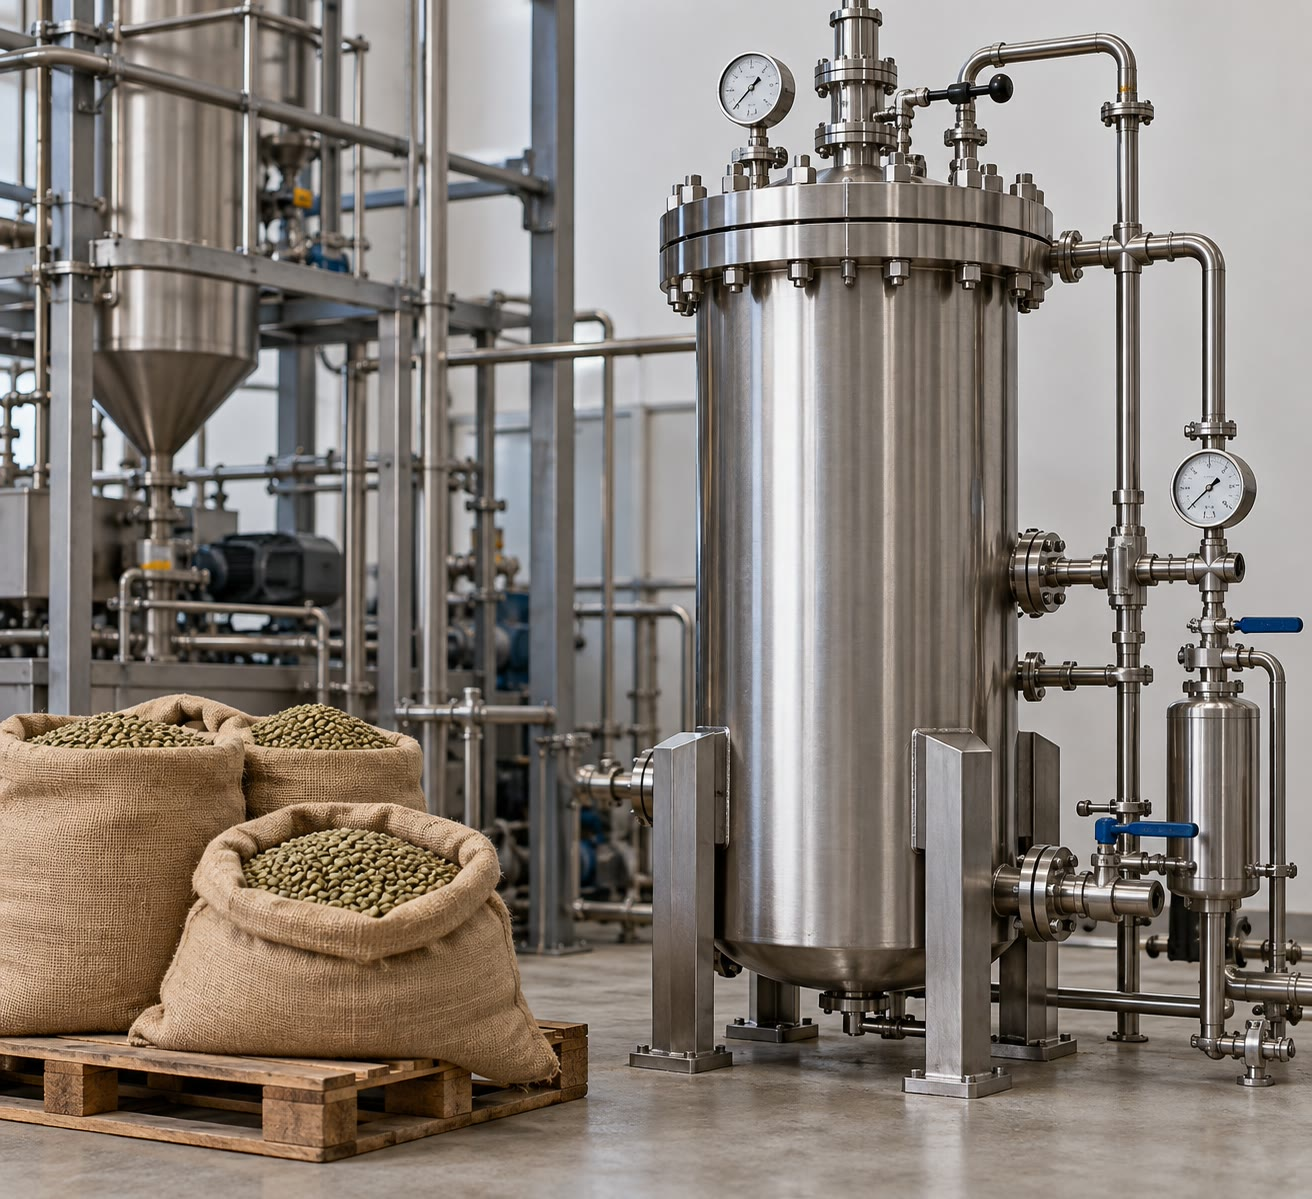
\includegraphics[width=0.45\linewidth,height=6cm,keepaspectratio]{images/book1/ai/g12-scco2-vessel.jpg}

{\small Un recipiente de \omterm{def:g10:chemical-species:extraction}{extracción} a alta presión, en el que el dióxido
de carbono supercrítico sustituye a un \omterm{def:g6:solutions-and-solubility:solute}{disolvente} orgánico.}
\end{omfigure}

\section{Ejercicios}

\begin{exercise}[$\star$]\label{exo:g12:synthesis-strategy:1}
El etanol puede fabricarse por hidratación del eteno,
\ce{C2H4 + H2O -> C2H5OH}, o por fermentación de la glucosa,
\ce{C6H12O6 -> 2C2H5OH + 2CO2}. Calcula la \omterm{def:g12:synthesis-strategy:atom-economy}{economía atómica} de cada
proceso.
\end{exercise}

\begin{exercise}[$\star$]\label{exo:g12:synthesis-strategy:2}
En el esquema del dipéptido de este capítulo, nombra la etapa en la que
se coloca cada \omterm{def:g12:synthesis-strategy:protecting-group}{grupo protector} y la etapa en la que se retira.
\end{exercise}

\begin{exercise}[$\star$]\label{exo:g12:synthesis-strategy:3}
Una fábrica sustituye un \omterm{def:g6:solutions-and-solubility:solute}{disolvente} clorado por agua en una de sus
reacciones. ¿Qué principio de la \omterm{def:g12:synthesis-strategy:green-chemistry}{química verde} aplica?
\end{exercise}

\begin{exercise}[$\star$]\label{exo:g12:synthesis-strategy:4}
¿Por qué un exceso de etanol aumenta el \omterm{def:g10:synthesis-yield:yield}{rendimiento} de una
esterificación, y un \omterm{def:g12:catalysis:catalyst}{catalizador} no?
\end{exercise}

\begin{exercise}[$\star$]\label{exo:g12:synthesis-strategy:5}
El borohidruro de sodio reduce los \omterm{def:g11:functional-groups:carbonyl}{aldehídos} y las \omterm{def:g11:functional-groups:carbonyl}{cetonas}, no los
\omterm{def:g11:functional-groups:carboxylic-acid}{ésteres}. ¿Es \omterm{def:g12:synthesis-strategy:chemoselective}{quimioselectiva} su reacción con el 4-oxopentanoato de
metilo (una \omterm{def:g11:functional-groups:carbonyl}{cetona} y un \omterm{def:g11:functional-groups:carboxylic-acid}{éster})? ¿Qué grupo cambia?
\end{exercise}

\begin{exercise}[$\star\star$]\label{exo:g12:synthesis-strategy:6}
Un \omterm{def:g10:the-mole:amount}{mol} de ácido etanoico y uno de etanol dan \qty{0.67}{mol} de \omterm{def:g11:functional-groups:carboxylic-acid}{éster} en
el equilibrio. Propón dos maneras de aumentar esta cantidad, y una de
alcanzarla más deprisa.
\end{exercise}

\begin{exercise}[$\star\star$]\label{exo:g12:synthesis-strategy:7}
El 4-oxopentanoato de metilo, \ce{CH3-CO-CH2-CH2-CO-O-CH3}, se trata una
vez con borohidruro de sodio y otra con un exceso de hidruro de litio y
aluminio, que reduce el \omterm{def:g11:functional-groups:carboxylic-acid}{éster} a dos \omterm{def:g11:functional-groups:alcohol}{alcoholes}. Escribe cada producto.
\end{exercise}

\begin{exercise}[$\star\star$]\label{exo:g12:synthesis-strategy:8}
En el diagrama de barras de las \omterm{def:g12:synthesis-strategy:atom-economy}{economías atómicas}, ¿qué reacciones
conservan más de tres cuartos de los \omterm{def:g7:atoms-and-molecules:atom}{átomos}? ¿Por qué factor es mejor la
ruta de tres etapas del ibuprofeno que la de seis?
\end{exercise}

\begin{exercise}[$\star\star$]\label{exo:g12:synthesis-strategy:9}
La aspirina se fabrica según \ce{C7H6O3 + C4H6O3 -> C9H8O4 + C2H4O2}.
Calcula su \omterm{def:g12:synthesis-strategy:atom-economy}{economía atómica} y la masa de subproducto por kilogramo de
aspirina.
\end{exercise}

\begin{exercise}[$\star\star$]\label{exo:g12:synthesis-strategy:10}
¿Por qué se calienta una \omterm{def:g10:synthesis-yield:synthesis}{síntesis} a reflujo y no en un matraz abierto?
¿Cuál de las dos cosas, la velocidad o el \omterm{def:g10:synthesis-yield:yield}{rendimiento}, mejora el
calentamiento?
\end{exercise}

\begin{exercise}[$\star\star$]\label{exo:g12:synthesis-strategy:11}
En la figura de las dos rutas del ibuprofeno, cuenta las etapas y di qué
principios de la \omterm{def:g12:synthesis-strategy:green-chemistry}{química verde} aplica la ruta nueva. Da tres.
\end{exercise}

\begin{exercise}[$\star\star\star$]\label{exo:g12:synthesis-strategy:12}
Una \omterm{def:g10:synthesis-yield:synthesis}{síntesis} de tres etapas tiene \omterm{def:g10:synthesis-yield:yield}{rendimientos} del \qty{80}{\percent},
del \qty{70}{\percent} y del \qty{90}{\percent}. Calcula el \omterm{def:g10:synthesis-yield:yield}{rendimiento}
global. ¿Qué cantidad de material de partida hace falta para obtener
\qty{0.10}{mol} de producto final, si un \omterm{def:g10:the-mole:amount}{mol} de material de partida da
como máximo un \omterm{def:g10:the-mole:amount}{mol} de producto?
\end{exercise}

\begin{exercise}[$\star\star\star$]\label{exo:g12:synthesis-strategy:13}
Planifica la \omterm{def:g10:synthesis-yield:synthesis}{síntesis} del dipéptido Ala--Gly (el ácido de la alanina
unido a la \omterm{def:g11:functional-groups:amine}{amina} de la glicina): ¿qué grupos proteges, y cuántas etapas
tiene el plan?
\end{exercise}

\begin{exercise}[$\star\star\star$]\label{exo:g12:synthesis-strategy:14}
Una empresa califica su proceso de ``verde'' porque usa un \omterm{def:g12:catalysis:catalyst}{catalizador}.
El proceso funciona a \qty{250}{\celsius} en benceno, un \omterm{def:g6:solutions-and-solubility:solute}{disolvente}
tóxico, y su \omterm{def:g12:synthesis-strategy:atom-economy}{economía atómica} es del \qty{35}{\percent}. Juzga la
afirmación, principio por principio.
\end{exercise}

\begin{exercise}[$\star\star\star$]\label{exo:g12:synthesis-strategy:15}
La cafeína se extrae de los granos de café con diclorometano, un
\omterm{def:g6:solutions-and-solubility:solute}{disolvente} clorado volátil, o con dióxido de carbono supercrítico a unos
\qty{40}{\celsius} y \qty{100}{bar}. Explica por qué el segundo es
supercrítico, por qué necesita un recipiente resistente, y da dos
ventajas que tiene sobre el primero.
\end{exercise}

\section{Problema: dos rutas hacia el ibuprofeno}

\begin{problem}[{Problema de fin de semana --- ¿cuántos residuos evita la ruta de
tres etapas por tonelada de ibuprofeno?}]
\label{pb:g12:synthesis-strategy:1}
% ledger: ibu:boots-ae, ibu:bhc-ae, ibu:boots-steps, ibu:bhc-steps, aw:C, aw:H, aw:O, aw:N, aw:Cl, aw:Na
La ruta antigua hacia el ibuprofeno \ce{C13H18O2} tiene seis etapas.
Sumados, sus \omterm{def:g7:chemical-reactions:reactant}{reactivos} son \ce{C10H14}, \ce{C4H6O3},
\ce{C4H7ClO2}, \ce{C2H5ONa}, un ácido contado como \ce{H3O},
\ce{NH3O} y dos \ce{H2O}. La ruta nueva tiene tres etapas:
\[
  \ce{C10H14 + C4H6O3 + H2 + CO -> C13H18O2 + C2H4O2} .
\]

\medskip
\noindent\textbf{Parte I --- Las ecuaciones.}
\begin{enumerate}
  \item Comprueba que la ecuación de la ruta nueva está ajustada en
        carbono, hidrógeno y oxígeno.
  \item Nombra el subproducto de la ruta nueva.
  \item En la ruta antigua, ¿qué elementos de los \omterm{def:g7:chemical-reactions:reactant}{reactivos} acaban por
        completo en los residuos?
  \item ¿Cuál de las dos rutas usa \omterm{def:g12:catalysis:catalyst}{catalizadores}? ¿Qué principio aplica
        eso?
\end{enumerate}

\medskip
\noindent\textbf{Parte II --- \omterm{def:g12:synthesis-strategy:atom-economy}{Economías atómicas}.}
\begin{enumerate}[resume]
  \item Calcula la \omterm{def:g10:the-mole:molar-mass}{masa molar} del ibuprofeno.
  \item Calcula la suma de las \omterm{def:g10:the-mole:molar-mass}{masas molares} de los \omterm{def:g7:chemical-reactions:reactant}{reactivos} de la ruta
        antigua.
  \item Deduce su \omterm{def:g12:synthesis-strategy:atom-economy}{economía atómica}.
  \item Calcula la suma de las \omterm{def:g10:the-mole:molar-mass}{masas molares} de los \omterm{def:g7:chemical-reactions:reactant}{reactivos} de la ruta
        nueva.
  \item Deduce su \omterm{def:g12:synthesis-strategy:atom-economy}{economía atómica}.
  \item ¿En cuánto se convierte si el ácido etanoico se cuenta como
        producto?
\end{enumerate}

\medskip
\noindent\textbf{Parte III --- Residuos por tonelada.}
\begin{enumerate}[resume]
  \item Para la ruta antigua, con un \omterm{def:g10:synthesis-yield:yield}{rendimiento} del \qty{100}{\percent},
        ¿qué masa de \omterm{def:g7:chemical-reactions:reactant}{reactivos} se compra por tonelada de ibuprofeno?
  \item ¿Qué masa de residuos da por tonelada?
  \item La misma pregunta para la ruta nueva: masa de \omterm{def:g7:chemical-reactions:reactant}{reactivos} por
        tonelada.
  \item Masa de ácido etanoico por tonelada.
  \item ¿Qué masa de residuos por tonelada se evita si el ácido etanoico
        se cuenta como residuo?
\end{enumerate}

\medskip
\noindent\textbf{Parte IV --- Los \omterm{def:g10:synthesis-yield:yield}{rendimientos} y el mundo real.}
\begin{enumerate}[resume]
  \item Supón que cada etapa tiene un \omterm{def:g10:synthesis-yield:yield}{rendimiento} del \qty{90}{\percent}.
        Calcula el \omterm{def:g10:synthesis-yield:yield}{rendimiento} global de la ruta antigua.
  \item Lo mismo para la ruta nueva.
  \item Da otra razón, además de la ecuación, por la que menos etapas
        significan menos residuos.
  \item En la práctica, el ácido etanoico se recupera y se aprovecha. ¿Qué
        masa de residuos por tonelada da entonces la ruta nueva, con un
        \omterm{def:g10:synthesis-yield:yield}{rendimiento} del \qty{100}{\percent}?
  \item Da la respuesta final: ¿cuántos residuos evita la ruta de tres
        etapas por tonelada de ibuprofeno?
\end{enumerate}
\end{problem}
